\section{Team and Roles}

Our team  is comprised of:
\begin{itemize}
\item Arthur Manoha
\item Louis Viot
\item Matthias Benkort
\item Matthieu Pizenberg
\item Nicolas Gaborit
\end{itemize}


We defined three specific roles within our team. These are the project
manager, the technical manager and the integration manager.

\begin{description}
\item[Technical Manager] \emph{(Matthias Benkort)} He is the one who
  has to know best the technologies we are using because he serves as
  a technical reference for the rest of the team. He is responsible
  for the overall architecture of the application and validates
  choices made in this regard. He is responsible for the overall
  quality of the code, including its extendibility and reusability. He
  also insure the overall consistency of the code by defining early on
  some coding style rules in a document called: Coding Style Guide.

\item[Integration Manager] \emph{(Matthieu Pizenberg)} He is the
  central part, insuring the code developed by everyone integrate well
  together without adding bugs. He setups the development environment
  (Git) and defines an integration process and a development workflow
  for this purpose. He is available to help everyone with the
  development tools.

\item[Project Manager] \emph{(Arthur Manoha then Nicolas Gaborit on
    week 5)} He is the team coordinator. He ensures good communication
  with the client and within the team. He establishes the planning and
  manage its evolution with the team. He also make sure a proper risk
  analysis is regularly made.
\end{description}


\section{Meetings}
We had two types of meeting throughout the project, the first with the
clients and the second with the industrial supervisor.

\subsection{Clients}
We met every Friday with the clients to present our progress, ask some
questions about problems we are facing or choices we are making, and
get a feedbacks from them. They lasted one hour and a half. However,
we tried not to wait until Friday when we needed to clarify things and
thus we used mails or video calls to communicate outside of this
schedule.

\subsection{Industrial Supervisor}
Every Tuesday was our weekly review with the industrial
supervisor. During those we reported on our progress and
difficulties. In particular, we discussed the hows and whys of tasks
related to project management : planning, specifications, risks and
response plan.

\section{Development environment}
\section{Quality insurance}

\section{Risks Management}
We made a formal risks analysis during the early weeks as a
brainstorming initally. We listed all the risks we could think of and
sorted them according to both their probability and impact. Then we
decided of a response plan or solution for each of them. This first
risks analysis is fully visible on page \pageref{fig:risks}. However,
we did not reiterated this process later. 

This resulted in some unexpected problems whose main consequences were
to add delay to the project:

\begin{description}
\item[No 3D optimisation in Python] The Python OpenGL bindings would
  not allow us to optimize the 3D rendering of the point cloud using
  \code{Vertex Array Objects} and \code{Buffer Objects}. So we needed
  to use \verb!C++! and make a QML plugin that could integrate in
  PyQt. Learning how to integrate a \verb!C++! plugin in PyQt took some time.
\item[Libraries installations] We tried to install the libraries we
  were using at the ENSEEIHT to allow everyone to work
  together. However it ended not being possible and some members of
  the team lost a few days in the process. We could have avoided that
  by analyzing first the risk involved and according us a deadline for
  the installations.
\end{description}

We did take some preventive actions though, but we did not formalized
it. For example, when we faced the necessity of using \verb!C++! Qt instead
of PyQt to develop the point cloud rendering QML plugin, we were not
certain of achieving this task in time. For this purpose, we developed
in parallel another faster, less satisfying solution.


\begin{figure}[!htbp]
  \centering
  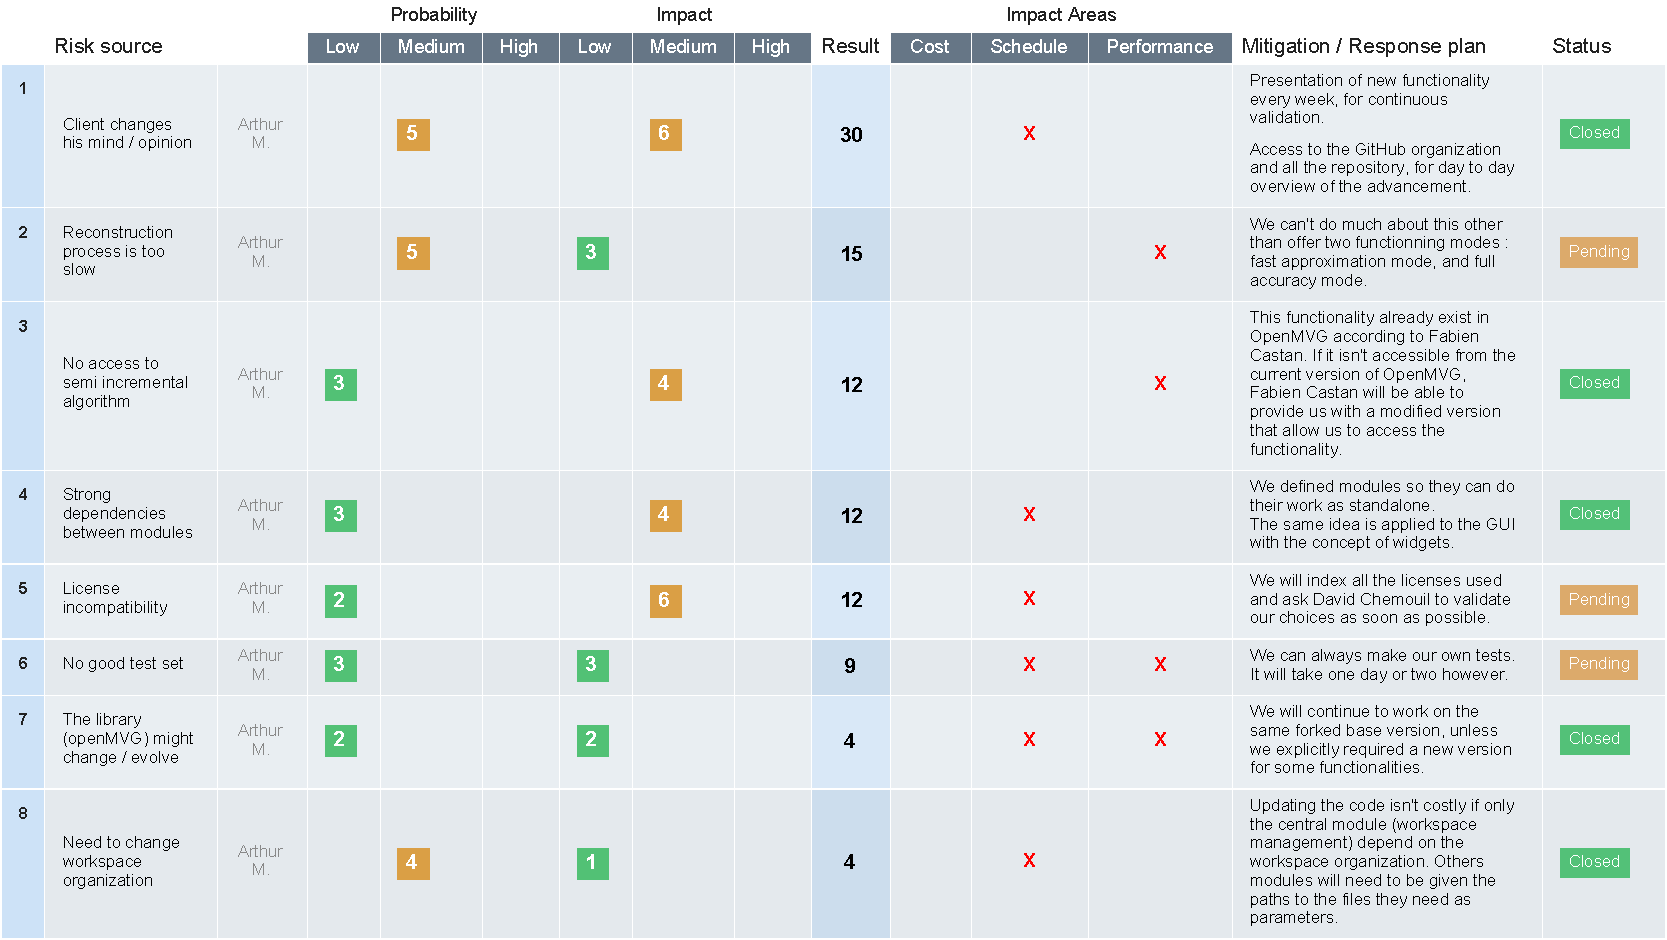
\includegraphics[width=\linewidth]{img/risks.pdf}
  \caption{Risks report on 3rd week}
  \label{fig:risks}
\end{figure}

\section{Planning}

Establishing a planning was the hardest project management task in the
project. First because we lacked the tools to work on PERT or Gantt
diagrams easily\ldots The one we used
(\href{https://www.teamwork.com/}{Teamwork}) was incomplete but we
figured it out too late. Second because we had so many technologies to
learn before knowing what we had to do. And that is indeed the point:
we should have planned our training period. The key is not to have a
fully detailed planning like the first one we came up with. The key is
to start small and refine the planning as the project goes. You will
find the planning we made on week 5 as an appendix on page
\pageref{app:planning}.
